\section{Teórico}

  \definicion{Topic:} Introduction to Magnetism.

  \definicion{Speaker:}	Alessandro STROPPA (CNR-SPIN, Italy).

\subsection{Integrales de Coulomb y de intercambio}

  La integral de Coulomb $I$ es una cantidad positiva que hace referencia a la repulsión electrostática entre las densidades electrónicas $\norm{\psi_{100} (\vec{r}_1)}^2$ y $\norm{\psi_{nlm} (\vec{r}_2)}^2$; en cambio, la integral de intercambio $J$ es la energía asociada al intercambio de los estados cuánticos entre 2 electrones. El valor de $J$ puede ser negativo (antiparalelos) o positivo (paralelos).

  En el caso del singlete la repulsión Coulómbica tiende a ser mayor debido a que los electrones están más cercanos entre sí. La diferencia etre el estado single y el triple es $2J$.
    \begin{figure}[H]
        \centering
        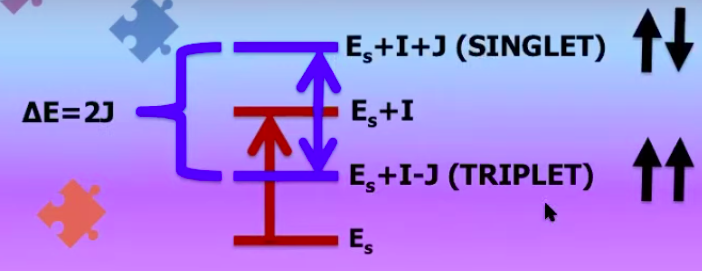
\includegraphics[scale = 0.6]{figs/D7/IJ.png}
    \end{figure}

  Cuando consideramos la interacción Coulómbica interelectrónica junto al postulado de simetrización llegamos al intercambio. Luego, partiendo desde un Hamiltoniano que no depende del spin podemos llegar a interacciones spin-dependientes.

\subsection{Interacción spin-órbita}

  La interacción spin-órbita (SO) es el acople entre el momento angular de spin $\vec{s}$ y el momento angular orbital $\vec{l}$. Esta interacción es unas 10 a 100 veces menor que el intercambio. A pesar de ser tan pequeña su  contribución es muy importante para el magnetismo.

  La energía magnética es $E = - \vec{m}_S \cdot \vec{B}_L$ y, como $\vec{m}_S \propto \vec{s}$ y $\vec{B}_L \propto \vec{l}$, entonces $E \propto \vec{s} \cdot \vec{l}$. El splitting generado por el acople SO puede ir desde los $10^{-5}$ eV para átomos livianos hasta los 0.1-1 eV para átomos pesados.

  La importancia del acople SO es que determina la anisotropia magnetocristalina en sólidos.

\subsection{High vs low spin}

  Al combinar el principio de exclusión de Pauli con las reglas de Hund, obtenemos dos situaciones:
    \begin{itemize}
      \item \textbf{High spin:} cuando la interacción $J$ es mayor que el splitting generado por el campo ligando, es preferible llenar la mayor cantidad de orbitales con igual spin (incluyendo orbitales de alta energía) antes de comenzar a utilizar el spin opuesto.
      \item \textbf{Low spin:} cuando la interacción $J$ es menor que el splitting generado por el campo ligando, es preferible llenar sólo los orbitales de menor energía.
    \end{itemize}

    \begin{figure}[H]
        \centering
        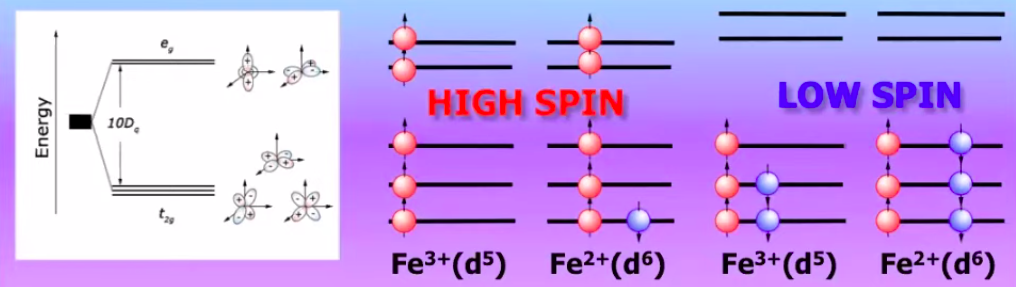
\includegraphics[scale = 0.5]{figs/D7/highlow.png}
    \end{figure}

\subsection{Potencial centrífugo: magnetismo localizado vs itinerante}

  Los electrones internos determinan el potencial sobre el cual se mueven los electrones externos. Este potencial central depende del momento angular orbital: a mayor $l$, más atrapados (localizados) estarán los electrones. Esto da lugar a la localización en los electrones 3d de los metales de transición y en los 4fde las tierras raras.

\subsection{Modelo de Stoner}

  Se trata del modelo de bandas más sencillo utilizado para explicar el ferromagnetismo en metales. La interacción entre los electrones 3d provoca un smearing de su energía, dando lugar a una banda, la cual puede describirse con DFT. Al considerar la energía media de los estados de la banda de valencia se puede aproximar la DOS mediante un semicírculo.

    \begin{figure}[H]
        \centering
        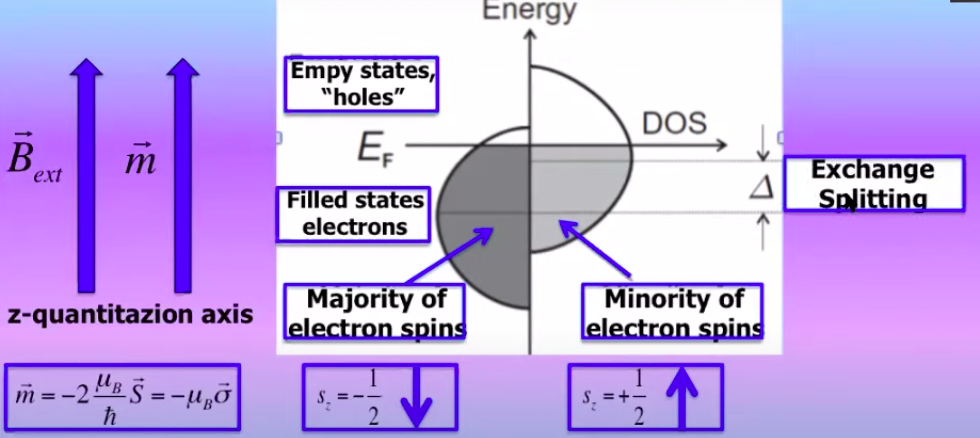
\includegraphics[scale = 0.5]{figs/D7/stoner.png}
    \end{figure}

\subsection{Magnetismo colineal y no colineal}

  En el caso no colineal no existe un único eje de cuantización principal, por lo que se deben generar CL entre los spins up y down; en cambio, en el caso colineal sí se tiene un único eje de cuantización principal permitiendo tener por un lado la contribución up y por otra parte la contribución down.

  \begin{figure}[H]
      \centering
      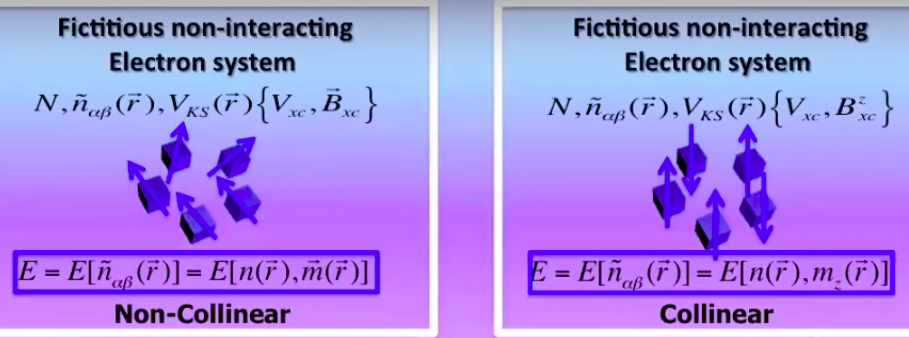
\includegraphics[scale = 0.5]{figs/D7/colin.png}
  \end{figure}

  Al final de cuentas tenemos que:
    \begin{itemize}
      \item La densidad de carga es la suma de las contribuciones up y down de la función de onda.
      \item La densidad de spin en $z$ es la resta de las contribuciones up y down de la función de onda.
      \item La densidad de spin en $x$ y en $y$ son la parte real y la parte imaginaria, respectivamente, del producto entre la función de onda y su conjugada, ambas con spins opuestos.
    \end{itemize}

\subsection{Spin DFT}

  Para hacer DFT considerando el spin hay que extender las ecuaciones KS a sistemas spin-polarizados, introduciendo una matriz 2x2 para la densidad electrónica. A partir de esto, las densidades y los potenciales se pueden descomponer como CL de las matrices de Pauli: la contribución escalar viene de DFT sin spin mientras que la contribución vectorial viene de la mano del magnetismo.

  En QE podemos obtener:
    \begin{itemize}
      \item Energía total (pw-scf).
      \item Momento magnético de spin total y absoluto  (pw-scf).
      \item Estructura de bandas (pw-nscf), tanto para el caso de spins no polarizados como para polarización colineal y no colineal.
      \item DOS (pw-nscf): DOS total o local.
      \item Momentos locales.
    \end{itemize}

\section{Q\&A}

  \definicion{can we calculate the exchange interaction using QE?}

  You may extract exchange interactions by fitting your results to some suitable spin hamiltonian; or, if you know the integrals to be computed, you can use data from QE to compute them. QE doesn't directly do that, though.

  \definicion{Why in the magnetic case in 'scf' calculation the flag 'starting\_magnetization' is 0.26, while in the 'nscf' one the flag 'starting\_magnetization' is set to 0.7?}

  It is just an initial guess (the important thing is that it is different from 0.0) and I add, in the ncsf run it does not compute again the magnetic moment- It just reads the charge  density and diagonalize the matrix to compute the dos

  \definicion{If we have 2 atoms in unit cell, we don’t have to specific starting\_magnetization(2)?}

  starting\_magnetization is set PER TYPE OF ATOM, not per atom

  \definicion{how can we specify nbnd in the input file?}

  Nbnd1 = no. of electrons/2 ; in order to know the information of un occupied states (x). Now nbnd = Nbnd1+x

  Generally 20\% larger than the number of  occupied states

\section{Hands-on}

  \definicion{Topic:} Introduction to Magnetism.

  \definicion{Speaker:}	Pietro DELUGAS (SISSA, Italy).

  Se estudia el magnetismo en metales de transición: Fe, Co y Ni.

\subsection{Ferromagnetismo en Fe BCC}

  Vamos a comparar las soluciones no magnética y ferromagnética (colineal) para el caso de Fe BCC. Para eso calcularemos las constantes de red óptimas en cada caso usando LDA. Luego, calcularemos DOS y PDOS de ambos casos utilizando el parámetro de red óptimo.

\subsubsection{Parámetro de red}

  Primero vamos a estudiar el parámetro de red para el caso no magnético. El script barre el parámetro de red y calcula las energías del estado fundamental. Luego, reúne los resultados en $energies.dat$. Posteriormente ejecutamos ev.x y respondemos las preguntas que nos hace:
    \begin{itemize}
      \item Lattice parameter or Volume are in (au, Ang): au.
      \item Enter type of bravais lattice (fcc, bcc, sc, noncubic): bcc.
      \item 1=birch1, 2=birch2, 3=keane, 4=murnaghan: 4.
      \item Input file: energies.dat.
      \item Output file: nonmag.out
    \end{itemize}

  El mínimo se obtiene a los 5.1070 Bohr.

  Para el caso mangético hacemos exactamente lo mismo. Como el cálculo es colineal, debemos agregar:
    \begin{itemize}
      \item $nspin=2$ indica que debe considerar polarización de spin colineal. Si fuera $1$ es que no hay polarización.
      \item $starting\_magnetization(1)=0.3$ rompemos la simetría entre los spins up y down. Esto da como resultado una magnetización inicial igual a 0.3 multiplicada por la carga de valencia del ion.
    \end{itemize}

  En el output aparecerá la mangnetización total (con signo) y la absoluta.
    \begin{figure}[H]
        \centering
        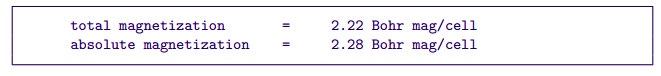
\includegraphics[scale = 0.6]{figs/D7/output_col.png}
    \end{figure}

  Si quisiéramos hacer un cálculo no colineal deberíamos agregar lo siguiente:
    \begin{itemize}
      \item $noncolin=.true.$ indica que queremos una polarización de spin no colineal.
      \item $starting\_magnetization$ para romper la simetría.
      \item $angle1(i)$ y $angle2(i)$ son los ángulos polar y acimutal, respectivamente, que determinan la dirección de la magnetización inicial para cada especie.
    \end{itemize}

    En el output aparecerá la mangnetización total (con signo y vectorial) y la absoluta.
      \begin{figure}[H]
          \centering
          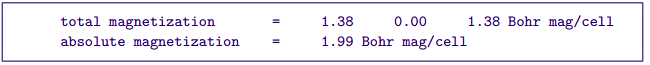
\includegraphics[scale = 0.6]{figs/D7/output_nocol.png}
      \end{figure}

    Además, en ambos casos aparecerá un estimado de la magnetización en cada sitio iónico, ya sea como una cantidad escalar o como una cantidad vectorial.
      \begin{figure}[H]
          \centering
          \subfigure[colineal]{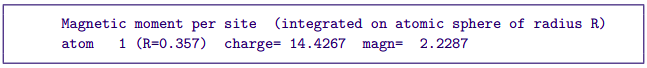
\includegraphics[scale = 0.6]{figs/D7/output_estim.png}}
          \subfigure[no colineal]{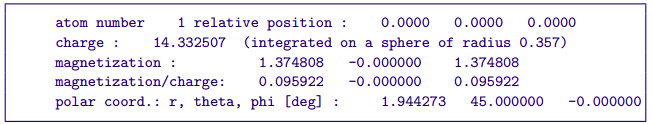
\includegraphics[scale = 0.6]{figs/D7/output_vec.png}}
      \end{figure}

    Luego de hacer los cálculos, el mínimo se obtiene a los 5.1969 Bohr. Dado que el hierro es una material magnético, vemos que la solución magnética tiene menor energía total por celda. Además, tiene un parámetro de red mayor. Sin embargo, LSDA subestima el parámetro de red: el dato experimental es 5.4 Bohr.
    \begin{figure}[H]
        \centering
        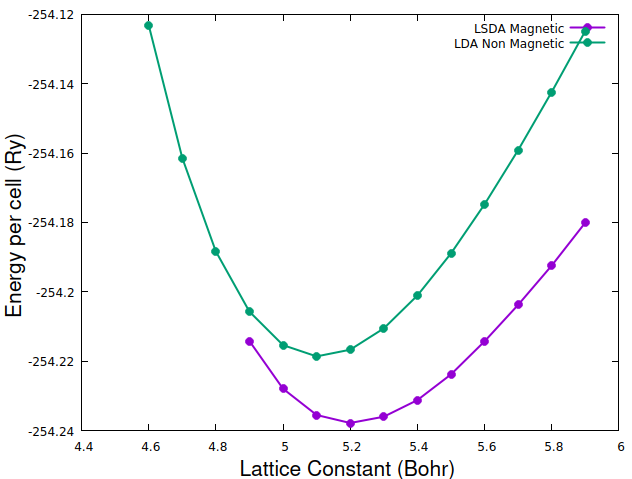
\includegraphics[scale = 0.6]{figs/D7/comparacion.png}
    \end{figure}

\subsubsection{DOS y PDOS: exchange splitting}

  Utilizando los parámetros de red óptimos para cada caso, vamos a determinar sus DOS. Vemos que se rompe la degeneración al considerar magnetismo: los spins up se corren hacia valores por debajo de la energía de Fermi y los spins down se corren a valores más altos.

  \begin{figure}[H]
      \centering
      \subfigure[no magnético]{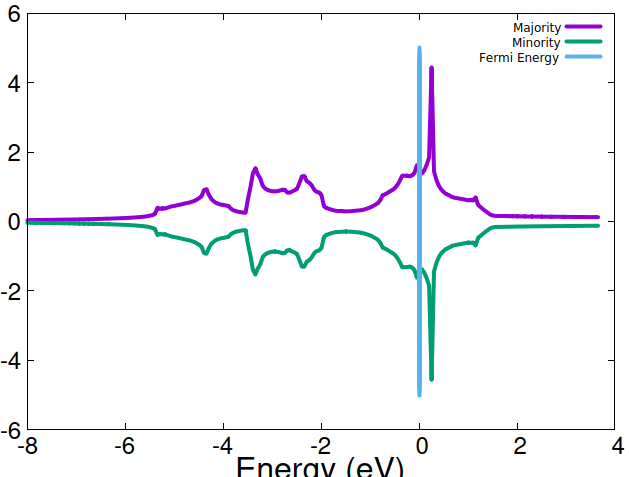
\includegraphics[scale = 0.6]{figs/D7/DOS_nomag.png}}
      \subfigure[magnético]{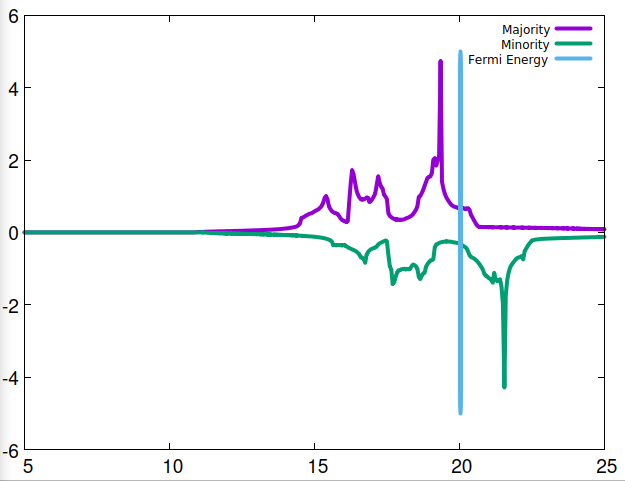
\includegraphics[scale = 0.6]{figs/D7/DOS_mag.png}}
  \end{figure}

  Vamos a corroborar que el exchange splitting está relacionado con la ocupación parcial del 3d del Fe: vemos claramente que la mayor contribución es del 3d.
  \begin{figure}[H]
      \centering
      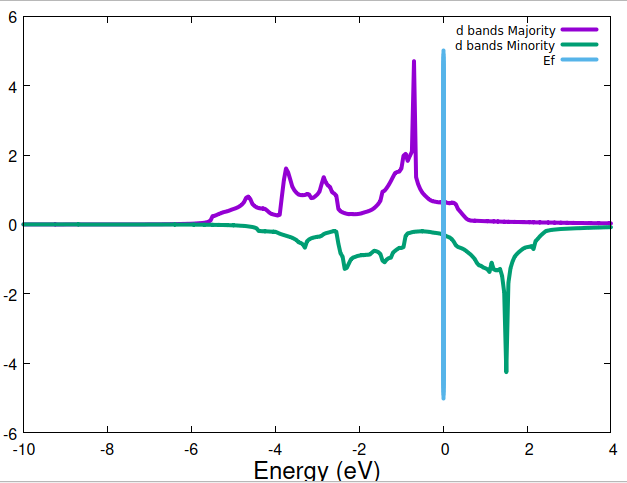
\includegraphics[scale = 0.6]{figs/D7/PDOS.png}
  \end{figure}

\subsubsection{Momento magnético bajo presión}

  Vamos a estudiar la evolución del momento magnético de Fe para diferentes parámetros de red: veremos con PDOS que tanto el exchange splitting como el momento magnético se reducen a medida que el material es comprimido.

  \Obs{Vamos a usar PBE en vez de LDA para tener parámetros de red más reales.}

  A medida que achicamos la red, la magnetización disminuye.
  \begin{figure}[H]
      \centering
      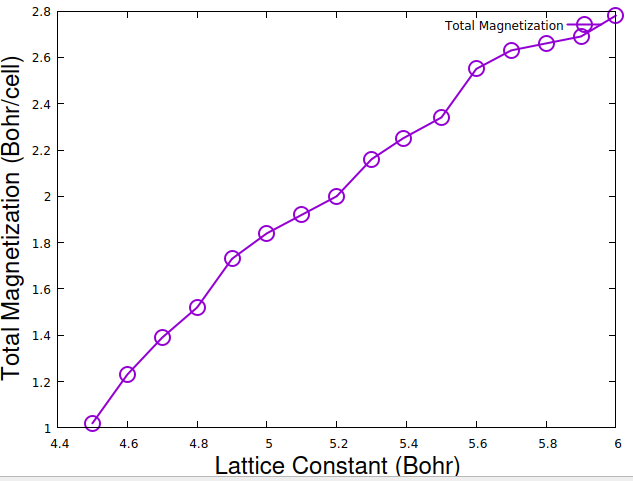
\includegraphics[scale = 0.6]{figs/D7/ex2.png}
  \end{figure}

\subsection{Magnetismo en metales de transición}

  Vamos a comparar las propiedades magnéticas de Fe BCC, Co HPC y Ni FCC.

  Primero vemos las DOS para cada caso.
  \begin{figure}[H]
      \centering
      \subfigure[Fe]{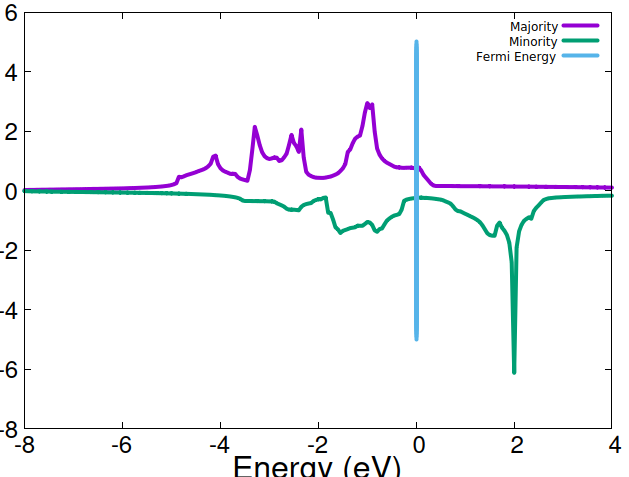
\includegraphics[scale = 0.6]{figs/D7/ex3_DOS_Fe.png}}
      \subfigure[Co]{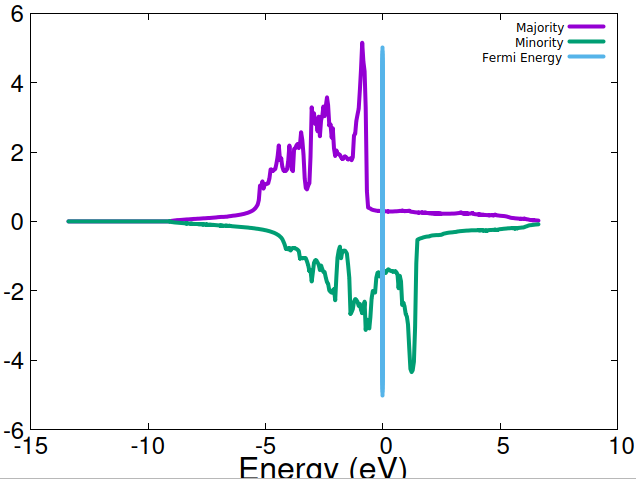
\includegraphics[scale = 0.6]{figs/D7/ex3_DOS_Co.png}}
      \subfigure[Ni]{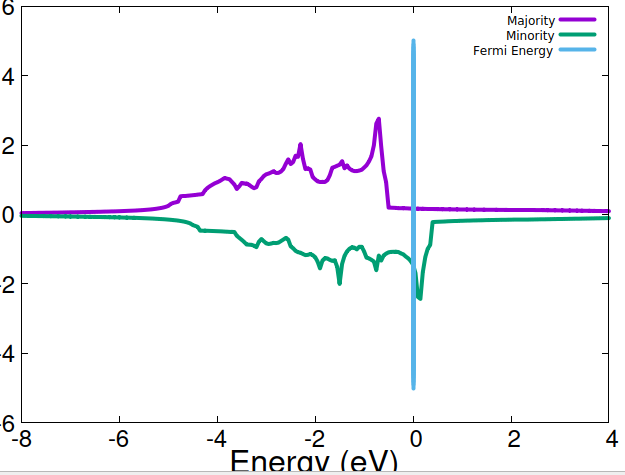
\includegraphics[scale = 0.6]{figs/D7/ex3_DOS_Ni.png}}
  \end{figure}

  Luego hacemos la PDOS. Al final de los pdos.out se tienen las lowdin charges donde describe cada átomo e indica su polarización: tanto el momento magnético total como las contribuciones parciales de cada orbital participante (según el PP).

  Resumen de resultados:
    \begin{itemize}
      \item total magnetization (SCF) Bohr magn/cell
        \begin{itemize}
          \item Fe    2.25
          \item Co    3.34  (2 atoms per cell)
          \item Ni    0.65
        \end{itemize}
      \item position of 3d pdos majoriy peak  w.r.t. Fermi Energy (eV)
        \begin{itemize}
          \item Fe  -0.91
          \item Co  -0.88
          \item Ni  -0.70
        \end{itemize}
      \item position of the 3d pdos minority peak w.r.t Fermi Energy (eV)
        \begin{itemize}
          \item Fe      +2.00
          \item Co      +1.24
          \item Ni      +0.15
        \end{itemize}
      \item Exch. splittings  (eV)
        \begin{itemize}
          \item Fe  2.91
          \item Co  2.12
          \item Ni  0.85
        \end{itemize}
      \item ion magnetization by Lowdin charges (`projwfc.x` output) in Bohr magn.
        \begin{itemize}
          \item Fe
              \begin{verbatim}
              polarization =   2.2245, s = -0.0197, p = -0.1266, d =  2.3707
              \end{verbatim}
           \item Co
           \begin{verbatim}
             polarization =   1.6457, s = -0.0196, p = -0.1288, d =  1.7941
           \end{verbatim}
           \item Ni
           \begin{verbatim}
             polarization =   0.6457, s = -0.0089, p = -0.0658, d =  0.7204
           \end{verbatim}
        \end{itemize}
    \end{itemize}

\subsection{Bandas en sistemas magnéticos: Ni FCC}

  Vamos a calcular las bandas de Ni FCC con polarización de spin para el caso colineal y el no colineal.
  \begin{figure}[H]
      \centering
      \subfigure[colineal]{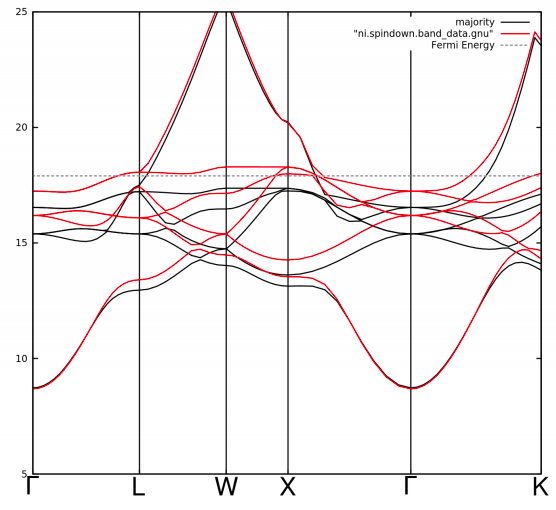
\includegraphics[scale = 0.6]{figs/D7/Ni_col.png}}
      \subfigure[nocolineal]{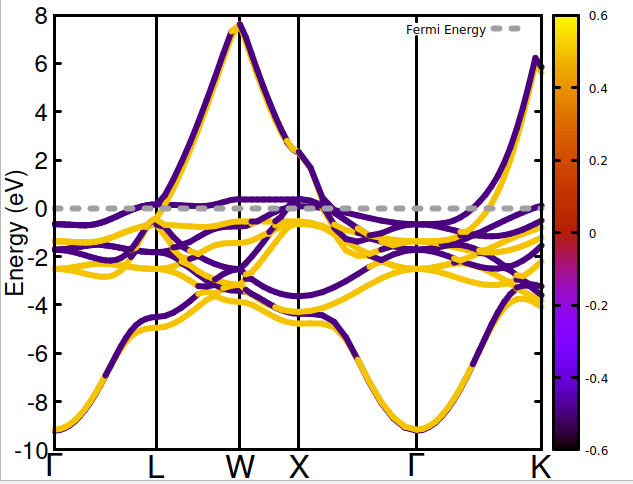
\includegraphics[scale = 0.6]{figs/D7/Ni_nocolin.png}}
  \end{figure}
